% !TeX root = ../main.tex


\begin{frame}
  \frametitle{{\small Coverage Testing for Topological  {\color{red} Scalar Field} Analysis}}

  \begin{textblock*}{12cm}(1cm,2cm)
    A real-valued function $f : D \to \R$.
  \end{textblock*}

  \begin{textblock*}{12cm}(1cm,5cm)
    
\includegraphics[trim=200 200 200 200, clip, width=0.5\textwidth]{../scripts/figures/surf/side_all.png}
    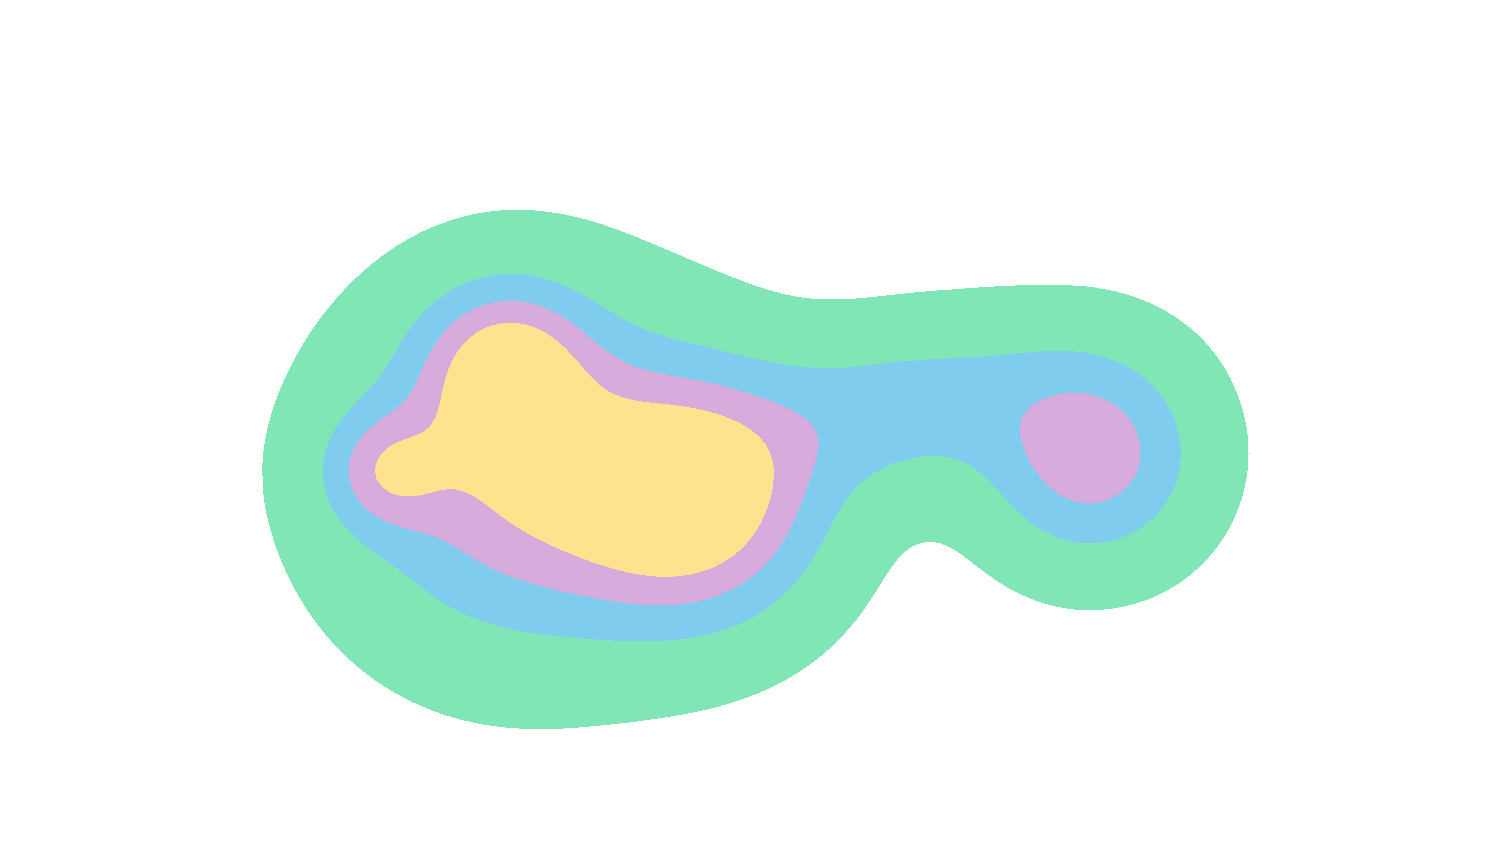
\includegraphics[trim=250 0 50 100, clip, width=0.4\textwidth]{../scripts/figures/surf/top_all.png}
  \end{textblock*}
\end{frame}

\begin{frame}
  \frametitle{{\small Coverage Testing for {\color{red} Topological Scalar Field Analysis}}}
  % How the \emph{shape} of $f^{-1}((-\infty,\alpha])$ changes with $\alpha\in\R$.
  \begin{textblock*}{12cm}(1cm,2cm)
    How the \emph{shape} of $f$ changes with $\alpha\in\R$.   \only<2>{$\alpha=0.2$}\only<3>{$\alpha=0.5$}\only<4>{$\alpha=0.8$}\only<5>{$\alpha=1$}
  \end{textblock*}

  \begin{textblock*}{12cm}(1cm,3cm)
    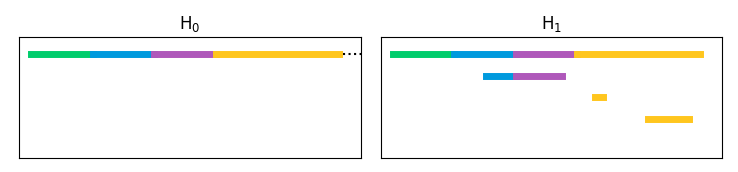
\includegraphics[width=0.6\textwidth]{../scripts/figures/scalar_barcode_true.png}
  \end{textblock*}

  \begin{textblock*}{12cm}(1cm,5cm)
    \includegraphics<1>[trim=200 200 200 200, clip, width=0.5\textwidth]{../scripts/figures/surf/side_all.png}
    \includegraphics<1>[trim=250 0 50 100, clip, width=0.4\textwidth]{../scripts/figures/surf/top_all.png}
    \includegraphics<2>[trim=200 200 200 200, clip, width=0.5\textwidth]{../scripts/figures/surf/side_B.png}
    \includegraphics<2>[trim=250 0 50 100, clip, width=0.4\textwidth]{../scripts/figures/surf/top_B.png}
    \includegraphics<3>[trim=200 200 200 200, clip, width=0.5\textwidth]{../scripts/figures/surf/side_C.png}
    \includegraphics<3>[trim=250 0 50 100, clip, width=0.4\textwidth]{../scripts/figures/surf/top_C.png}
    \includegraphics<4>[trim=200 200 200 200, clip, width=0.5\textwidth]{../scripts/figures/surf/side_D.png}
    \includegraphics<4>[trim=250 0 50 100, clip, width=0.4\textwidth]{../scripts/figures/surf/top_D.png}
    \includegraphics<5>[trim=200 200 200 200, clip, width=0.5\textwidth]{../scripts/figures/surf/side_all.png}
    \includegraphics<5>[trim=250 0 50 100, clip, width=0.4\textwidth]{../scripts/figures/surf/top_all.png}
  \end{textblock*}
\end{frame}

\begin{frame}
  \frametitle{{\small {\color{red} Coverage Testing} for Topological Scalar Field Analysis}}

  \begin{textblock*}{12cm}(1cm,2cm)
    \only<1>{Sample $P\subset D$ of $f : D\to \R$.}
    \only<2>{Cover $P^\delta = \displaystyle\bigcup_{p\in P}\ball^\delta(p)$.}
    \only<3>{Discrete representation $\rips^\delta(P)$.}
    \only<4>{Use $\rips^\delta(P)$ to analyze $f$.}
  \end{textblock*}

  \begin{textblock*}{12cm}(1cm,4cm)
    \includegraphics<1>[trim=200 600 200 800, clip, width=0.5\textwidth]{../scripts/figures/samples/samples}
    \includegraphics<2>[trim=200 600 200 800, clip, width=0.5\textwidth]{../scripts/figures/samples/cover}
    \includegraphics<3>[trim=200 600 200 800, clip, width=0.5\textwidth]{../scripts/figures/samples/complex1}
    \includegraphics<4>[trim=200 600 200 800, clip, width=0.5\textwidth]{../scripts/figures/samples/scalar1}
  \end{textblock*}
\end{frame}

\begin{frame}
  \frametitle{{\small The Topological Coverage Criterion (TCC)}}

  \begin{textblock*}{12cm}(1cm,2cm)
    \only<1>{Bounded domain $D$ with boundary $B$.}
    \only<2>{Geometric sample of $D$.}
    \only<3>{Labeled points $Q\subset P$ in $B^{2\delta}$.}
    \only<4,5>{Determine coverage of $D\setminus B^{2\delta}$ from $\rips^\delta(P, Q)$.}
  \end{textblock*}

  \begin{textblock*}{12cm}(1cm,4cm)
    \includegraphics<1>[trim=200 600 200 800, clip, width=0.5\textwidth]{../scripts/figures/nocover/surf}
    \includegraphics<2>[trim=200 600 200 800, clip, width=0.5\textwidth]{../scripts/figures/nocover/samples}
    \includegraphics<3>[trim=200 600 200 800, clip, width=0.5\textwidth]{../scripts/figures/nocover/cover}
    \includegraphics<4>[trim=200 600 200 800, clip, width=0.5\textwidth]{../scripts/figures/nocover/complex}
    \includegraphics<5>[trim=200 600 200 800, clip, width=0.5\textwidth]{../scripts/figures/cover/complex}
  \end{textblock*}
\end{frame}

\begin{frame}
  \frametitle{{\small TCC $\to$ SFA}}

  \begin{textblock*}{12cm}(1cm,2cm)
    \only<1,2>{Consider partial coverage,}
    \only<2>{and suppose points sample some function $f : D\to \R$.}
    \only<3>{Define our boundary as a sublevel set $B_\omega$ of $f$.}
    \only<4>{Determine coverage of $D\setminus B_\omega$ from $\rips^\delta(P, Q)$.}
  \end{textblock*}

  \begin{textblock*}{12cm}(1cm,4cm)
    \includegraphics<1>[trim=200 600 200 800, clip, width=0.5\textwidth]{../scripts/figures/partial/complex}
    \includegraphics<2>[trim=200 600 200 800, clip, width=0.5\textwidth]{../scripts/figures/partial1/samples}
    \includegraphics<3>[trim=200 600 200 800, clip, width=0.5\textwidth]{../scripts/figures/partial2/samples}
    \includegraphics<4>[trim=200 600 200 800, clip, width=0.5\textwidth]{../scripts/figures/partial2/complex}
    % \includegraphics<3>[trim=200 600 200 800, clip, width=0.5\textwidth]{../scripts/figures/nocover/cover}
    % \includegraphics<4>[trim=200 600 200 800, clip, width=0.5\textwidth]{../scripts/figures/nocover/complex}
    % \includegraphics<5>[trim=200 600 200 800, clip, width=0.5\textwidth]{../scripts/figures/cover/complex}
  \end{textblock*}
\end{frame}

\begin{frame}
  \frametitle{{\small {\color{red} \textbf{Goal:}} Analyze $f$ where we have confirmed coverage.}}

  \begin{textblock*}{12cm}(1cm,2cm)
    \begin{enumerate}
      \item<2,3> Check for coverage of $D\setminus B_\omega$,
      \item<3> analyze $f$ in $D\setminus B_\omega$.
    \end{enumerate}
  \end{textblock*}

  \begin{textblock*}{12cm}(1cm,4cm)
    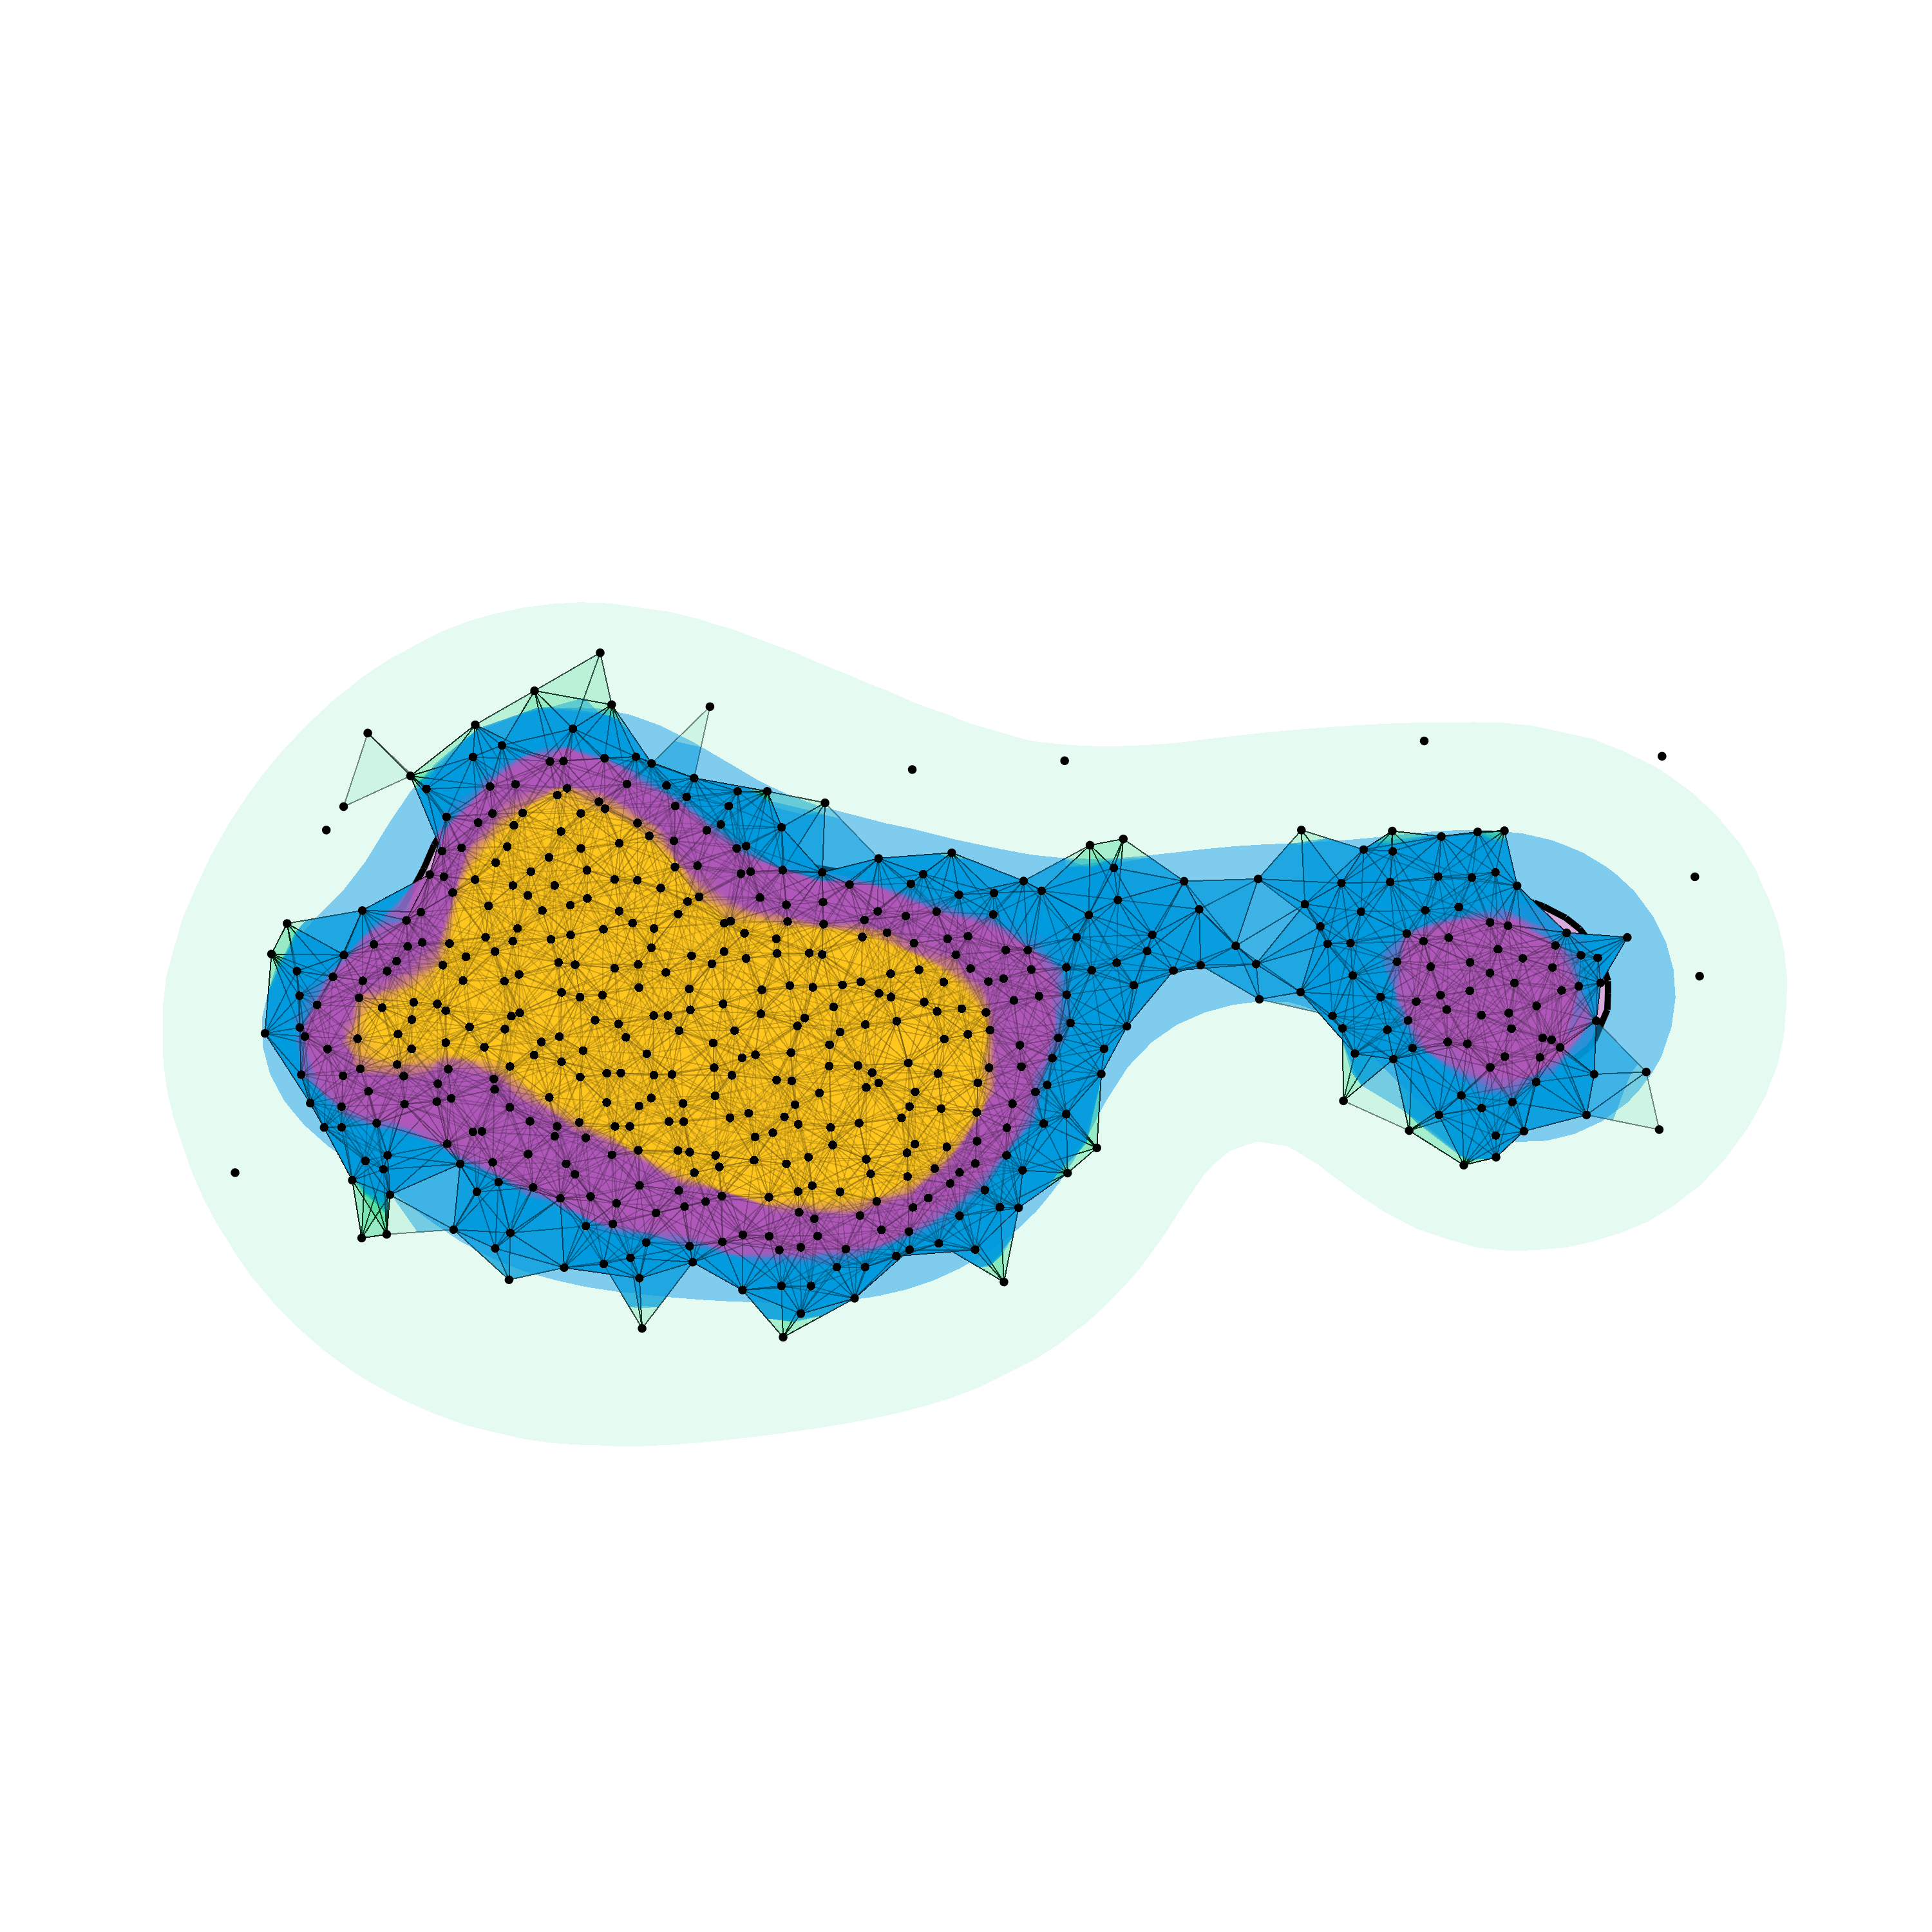
\includegraphics[trim=200 600 200 800, clip, width=0.5\textwidth]{../scripts/figures/samples/scalar1}
  \end{textblock*}
\end{frame}
